
\subsection{Description du transitoire}
Le bain initial correspond à un bain oxyde avec une masse initiale de 10t, une température initiale de 2900 K et une composition en fractions massiques de 0.77 UO$_2$ - 0.12 Zr - 0.11 ZrO$_2$ (ratio molaire $R_{U/Zr}$ = 1.3 et degré d'oxydation du zirconium $C_{Zr}$ = 30 \%). La puissance résiduelle massique est constante à $200$ W par kg d'uranium. Une condition adiabatique est imposée en surface haute de la couche d'acier liquide hors équilibre du bain (FE.). Un profil de flux plat est utilisé pour la distribution latérale de flux de toutes les couches du bain pour la projection des flux des différentes couches du bain sur les mailles de le croûte (voir section~\ref{sect:couplage}). Enfin, les caractéristiques utiles des différentes couches du bain sont détaillées dans le tableau~\ref{tab:caracteristiques_couches_bain}, en particulier les températures de ``liquidus'' des couches ainsi que les corrélations de flux de chaleur utilisées pour le calcul des puissances latérales $\phi S$ (voir~\cite{Bonnet1999} ou~\cite{Tourniaire2009a} pour plus de détails sur les corrélations).
\begin{table}
	\centering
	\begin{tabular}{ccc} 
	\hline
	Couche & $\temperature{liq}$ (K) & Corrélation latérale\\
	\hline
	Acier liquide (FE.) & 1600 & ChurchillAndChu\\
	Métal léger (LM.) & 1600 & ChurchillAndChu\\
	Oxyde (OX.) & 3000 & BaliDownWard\\
	Métal lourd (HM.) & 1600 & BaliDownWard\\
	\hline
	\end{tabular}	
	\caption{Caractéristiques de couches du bain pour le test} 
	\label{tab:caracteristiques_couches_bain}
\end{table}

Enfin, la croûte est divisée, tout au long du calcul, en 20 mailles. L'épaisseur de croûte ``résiduelle'' à son apparition est fixée à 5 mm. Une température constante et uniforme de 1600 K est imposée sur les parois extérieures de la croûte (seul le couplage entre le modèle de bain de corium et le modèle de croûte sont testés ici).

Une fois que ce bain oxyde et sa croûte ont atteint un régime permanent, une coulée d'acier liquide est considérée. La masse d'acier ajoutée a été selectionnée vis-à-vis du seuil d'inversion de stratification du bain\footnote{correspondant à quantité d'acier dans la bain permettant le passage d'un état d'équilibre thermochimique composé d'une couche métallique lourde en dessous d'une couche oxyde vers un équilibre composé d'une couche oxyde en dessous d'une couche métallique légère} afin d'amener le bain vers un équilibre à deux couche : une couche métallique lourde surmontée d'une couche oxyde. Les caractéristiques de cette coulée (temps de début et de fin, masse, température et composition) sont détaillés dans le tableau~\ref{tab:coulees_acier}. 
\begin{table}
	\centering
	\begin{tabular}{ccccc} 
	\hline
	$t_{\text{début}}$ (s) &  $t_{\text{arrêt}}$ (s) & Débit (kg/s) & T (K) & Composition\\
	\hline
	15 000 & 15 200 & 5 & 1605 & 0.687 Fe - 0.208 Cr - 0.106 Ni\\
	\hline
	\end{tabular}	
	\caption{Coulée d'acier liquide imposée pour le test} 
	\label{tab:coulees_acier}
\end{table}
A l'issue de cette coulée, un temps de simulation suffisamment long a été imposé pour permettre au bain d'atteindre un état thermique et thermochimique quasi-stationnaire. 

\subsection{Résultats et discussion}

L'état initial du bain ainsi que les différentes configurations quasi-stationnaires du bain obtenues (OX. puis HM./OX) sont décrites à la figure~\ref{fig:stratification_bains}.
\begin{figure}
\centering
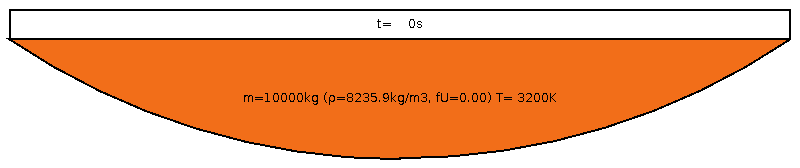
\includegraphics[width=0.8\textwidth, keepaspectratio=true]{Figures/coriumPool_t=00000.png}\\
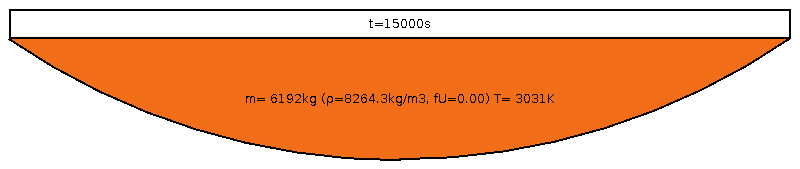
\includegraphics[width=0.8\textwidth, keepaspectratio=true]{Figures/coriumPool_t=15000.png}\\
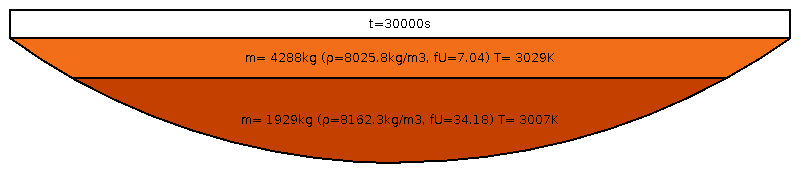
\includegraphics[width=0.8\textwidth, keepaspectratio=true]{Figures/coriumPool_t=30000.png}
\caption{La configuration initiale et les différentes stratifications quasi-stationnaires du bain de corium en fond de cuve atteintes lors du test : \textcolor{orange!75!black}{\textbf{OX.}} à t=15 000 s puis \textcolor{red!50!black}{\textbf{HM.}}/\textcolor{orange!75!black}{\textbf{OX.}} à t=30 000 s}
\label{fig:stratification_bains}
\end{figure}

% Par la suite, les premiers macro pas de temps du calcul ne seront pas considérés. L'initialisation thermique de la croûte expliquée dans la section~\ref{sect:thermique} permet effectivement d'obtenir un flux externe de croûte initialement nul. Néanmoins, la configuration du couplage thermique entre le bain de corium et la croûte amène le modèle de conduction 0D utilisé à sur-évaluer ce flux externe sur les pas de temps suivants. Néanmoins, au bout de quelques pas de temps (après épaississement de la croûte), le modèle de conduction évalue correctement les différents flux de chaleur de la croûte. Ces difficultés liées au modèle de conduction utilisé dans PROCOR ont déjà été identifiées dans une étude sur la prise en compte de la conduction axiale dans ce modèle dans~\cite{Peybernes2018} et des travaux sont en cours pour les soulever.

Durant les différentes étapes du transitoire, de la masse est échangée entre le bain de corium et sa croûte par solidification du bain ou fusion de la croûte. On notera que, comme le montre la figure~\ref{fig:stratification_bains}, le volume de la croûte est bien pris en compte pour le calcul du volume qu'occupe le bain de corium en fond de cuve de sorte que, le déplacement du niveau haut du bain associé à la solidification/fusion de la croûte (effet de densité) est faible.

La figure~\ref{fig:mass_balance} donne les masses des différentes couches du bain de corium et la masse globale de croûte.
\begin{figure}[H]
\centering
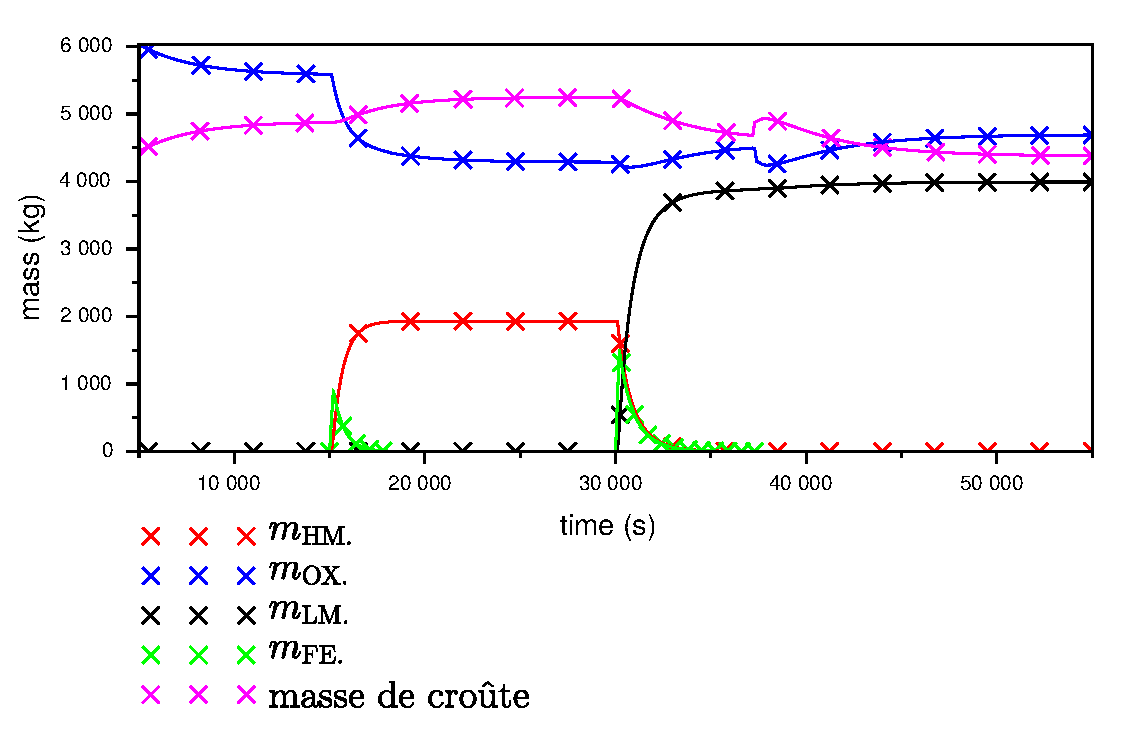
\includegraphics[width=0.85\textwidth, keepaspectratio=true]{Figures/mass_balance.eps}\\
\caption{Masses de la croûte et des couches du bain}
\label{fig:mass_balance}
\end{figure}
À chaque macro pas de temps du calcul et en fin de calcul, \emph{on vérifie bien la conservation de la masse globale du système}.

De la même manière, de l'énergie est échangée entre le bain de corium et la croûte et \emph{on vérifie la conservation globale de l'énergie du système}. La figure~\ref{fig:thermal_balance} donne les différentes puissances d'intérêt du bain de corium et de la croûte au cours du transitoire : les puissances évacuées par les surfaces latérales des différentes couches du bain $\bar{\phi}^{lat}_\textrm{HM.}S^{lat}_\textrm{HM.}$, $\bar{\phi}^{lat}_\textrm{OX.}S^{lat}_\textrm{OX.}$ et par sa surface supérieure $\bar{\phi}^{up}_\textrm{OX.}S^{up}_\textrm{OX.}$, la somme des puissances résiduelles des couches du bain $Q_\textrm{OX.}+Q_\textrm{HM.}$ ainsi que la somme des puissances résiduelles $Q_{C_j}$ des mailles $C_j$ de la croûte, et enfin la somme des puissances $\bar{\phi}_{j,ext}S_{j,ext}$ évacuées par la surface extérieure $\gamma_{ext}$ des mailles $C_j$ de la croûte.
\begin{figure}[H]
\centering
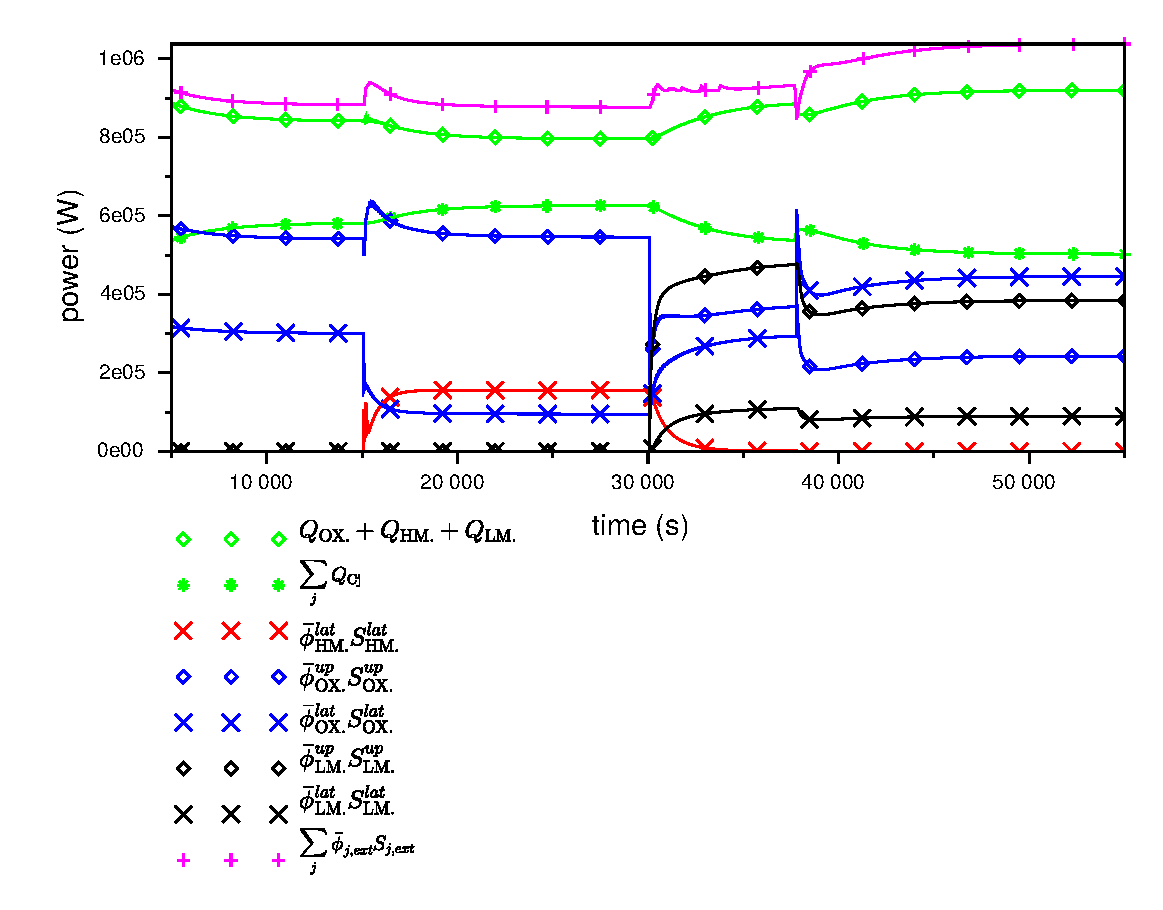
\includegraphics[width=0.85\textwidth, keepaspectratio=true]{Figures/thermal_balance.eps}\\
\caption{Puissances d'intérêt du système bain de corium et croûte}
\label{fig:thermal_balance}
\end{figure}
La conservation de l'énergie peut être vérifiée graphiquement dans la figure~\ref{fig:thermal_balance} aux deux états quasi-stationnaires atteints. Par exemple, pour t=15 000 s, on a :
\begin{equation}
\bar{\phi}^{up}_\textrm{OX.}S^{up}_\textrm{OX.} + \bar{\phi}_{j,ext}S_{j,ext} = Q_\textrm{OX.} + \sum_j Q_{C_j}.
\end{equation}

Durant le transitoire, les mailles de la croûte passent dans les différents états décrits dans la section~\ref{sect:thermique} (solidification, conduction et fusion). En particulier, pour la première partie du transitoire pour t $\leq$ 15 000 s, la croûte se solidifie jusqu'à atteindre un état quasi-stationnaire de solidification (voir figure~\ref{fig:croutes_1}) et, conformément au choix d'un profil uniforme de flux, l'épaisseur de la croûte est, elle aussi uniforme.

Lors de la seconde partie du transitoire, la couche de métal lourd apparaît suite à une coulée d'acier liquide (voir tableau~\ref{tab:coulees_acier}). La figure~\ref{fig:croutes_2} donne les différents états de la croûte durant ce transitoire.

Entre t=15 000 s et t=15 100 s, une maille de croûte apparaît en face d'une couche d'acier liquide (à une hauteur h $>$ 0.42 m) provenant de la coulée et le maillage de la croûte oxyde passe de 20 mailles (à t=15 000s) à 19 mailles (à t=15 100s). Cette maille de croûte acier apparaît avec une épaisseur initiale de 5 mm mais fond presque instantanément et disparaît. Ensuite, la couche de métal lourd s'épaissit et le volume du bain composé des couches HM. et OX. augmente du fait du transfert de masse depuis la couche FE. Par conséquent, une croûte oxyde apparaît au fur et à mesure que la couche OX. monte (voir les figures à t=16 000 s et t=18 000 s). Par ailleurs, comme attendu, en face de la couche HM., le flux latéral est évacué par conduction (sans évolution de la croûte oxyde). A t=30 000 s, la thermochimie et la thermique du bain se sont stabilisées et la croûte n'évolue plus : on retrouve bien les profils plats de flux de bain projetés sur les mailles de la croûte.

\begin{figure}[H]
\centering
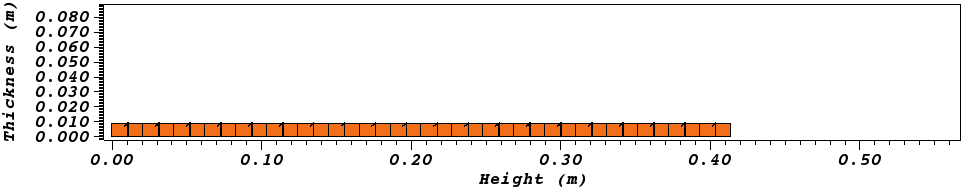
\includegraphics[width=\textwidth, keepaspectratio=true]{Figures/croute_100.png}\\
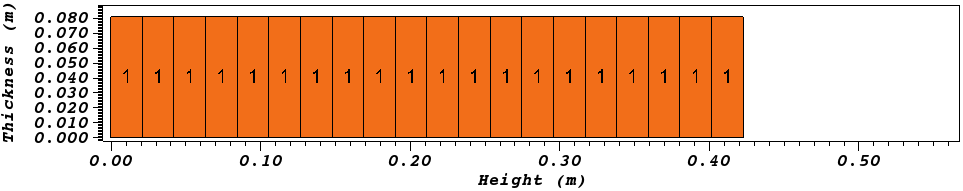
\includegraphics[width=\textwidth, keepaspectratio=true]{Figures/croute_15000.png}
\caption{Croûte à t = 100 s (en haut) et à t = 15 000 s (en bas). \textit{L'indice dans la maille $C_j$ donne la couche de bain en face de celle-ci : 0 $\Leftrightarrow$ HM., 1 $\Leftrightarrow$ OX.}}
\label{fig:croutes_1}
\end{figure}

\begin{figure}[H]
\centering
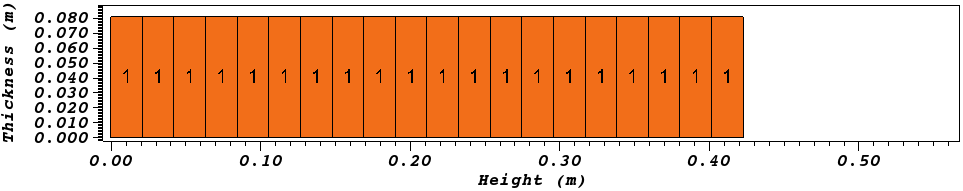
\includegraphics[width=\textwidth, keepaspectratio=true]{Figures/croute_15000.png}\\
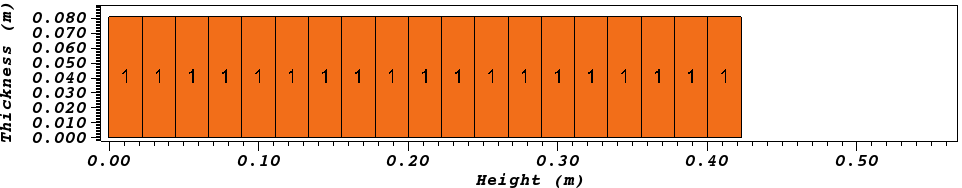
\includegraphics[width=\textwidth, keepaspectratio=true]{Figures/croute_15100.png}\\
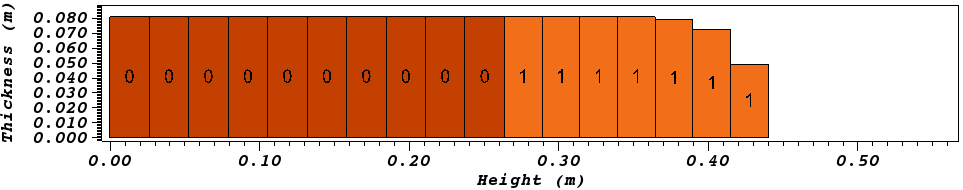
\includegraphics[width=\textwidth, keepaspectratio=true]{Figures/croute_16000.png}\\
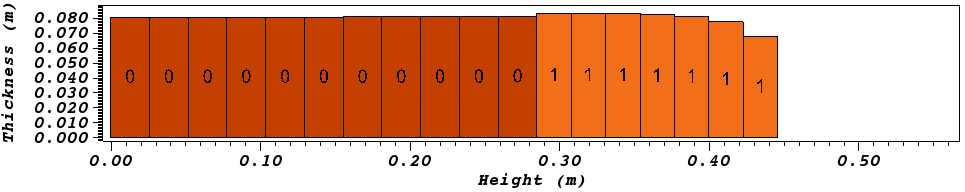
\includegraphics[width=\textwidth, keepaspectratio=true]{Figures/croute_18000.png}\\
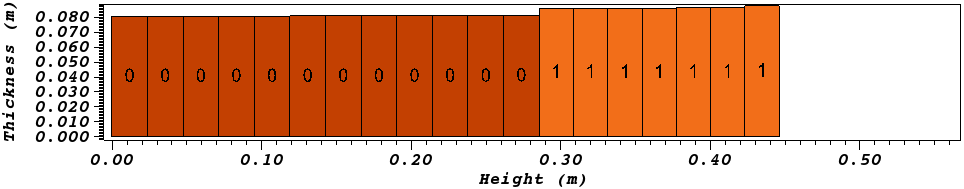
\includegraphics[width=\textwidth, keepaspectratio=true]{Figures/croute_30000.png}\\
\caption{De haut en bas, croûte à t = 15 000 s, t=15 100 s, t=16 000 s, t=18 000 s, t=30 000 s (état quasi-stationnaire du bain HM./OX.). \textit{L'indice dans la maille $C_j$ donne la couche de bain en face de celle-ci : 0 $\Leftrightarrow$ HM., 1 $\Leftrightarrow$ OX.}}
\label{fig:croutes_2}
\end{figure}
